\documentclass[11pt]{article}
\usepackage{geometry}                % See geometry.pdf to learn the layout options. There are lots.
\geometry{letterpaper}                   % ... or a4paper or a5paper or ... 
%\geometry{landscape}                % Activate for for rotated page geometry
%\usepackage[parfill]{parskip}    % Activate to begin paragraphs with an empty line rather than an indent
\usepackage{fancyhdr}
\usepackage{amsmath,amsfonts,amsthm,amssymb}
\usepackage{graphicx}
\usepackage{soul,color}
\usepackage{graphicx,float,wrapfig}
\usepackage{lastpage}
\usepackage{epstopdf}
\DeclareGraphicsRule{.tif}{png}{.png}{`convert #1 `dirname #1`/`basename #1 .tif`.png}

% Homework Specific Information
\newcommand{\hmwkTitle}{Homework 4}
\newcommand{\hmwkDueDate}{April 25, 2012}
\newcommand{\hmwkClass}{Computational Neuroscience}
\newcommand{\hmwkClassInstructor}{John Rinzel}
\newcommand{\hmwkAuthorName}{Raphael Sofaer}

% Setup the header and footer
\pagestyle{fancy}                                                       %
\lhead{\hmwkAuthorName}                                                 %
\rhead{\hmwkClass\ (\hmwkClassInstructor): \hmwkTitle}  %
\lfoot{\lastxmark}                                                      %
\cfoot{}                                                                %
\rfoot{Page\ \thepage\ of\ \pageref{LastPage}}                          %
\renewcommand\headrulewidth{0.4pt}                                      %
\renewcommand\footrulewidth{0.4pt}                                      %
\setlength{\headheight}{13.6pt}

\title{\large{\hmwkAuthorName}\vspace{0.1in}\\\textmd{\textbf{\hmwkClass:\ \hmwkTitle}}\\\normalsize\vspace{0.1in}\small{Due\ on\ \hmwkDueDate}\\\vspace{0.1in}\large{\textit{\hmwkClassInstructor}}\vspace{-0.5in}}
\author{}
\date{}
  
\begin{document}
\maketitle

\section*{Short-Term Memory model with Adaptation: 1}
I based my Matlab script (run in Octave) on STM\_MF.m.
For the first run, I used $\gamma=2$ to match the graph in the homework description.
With $\gamma=1$, A(t) increased more slowly, and
therefore took longer to grow large enough to drive down r(t).\\
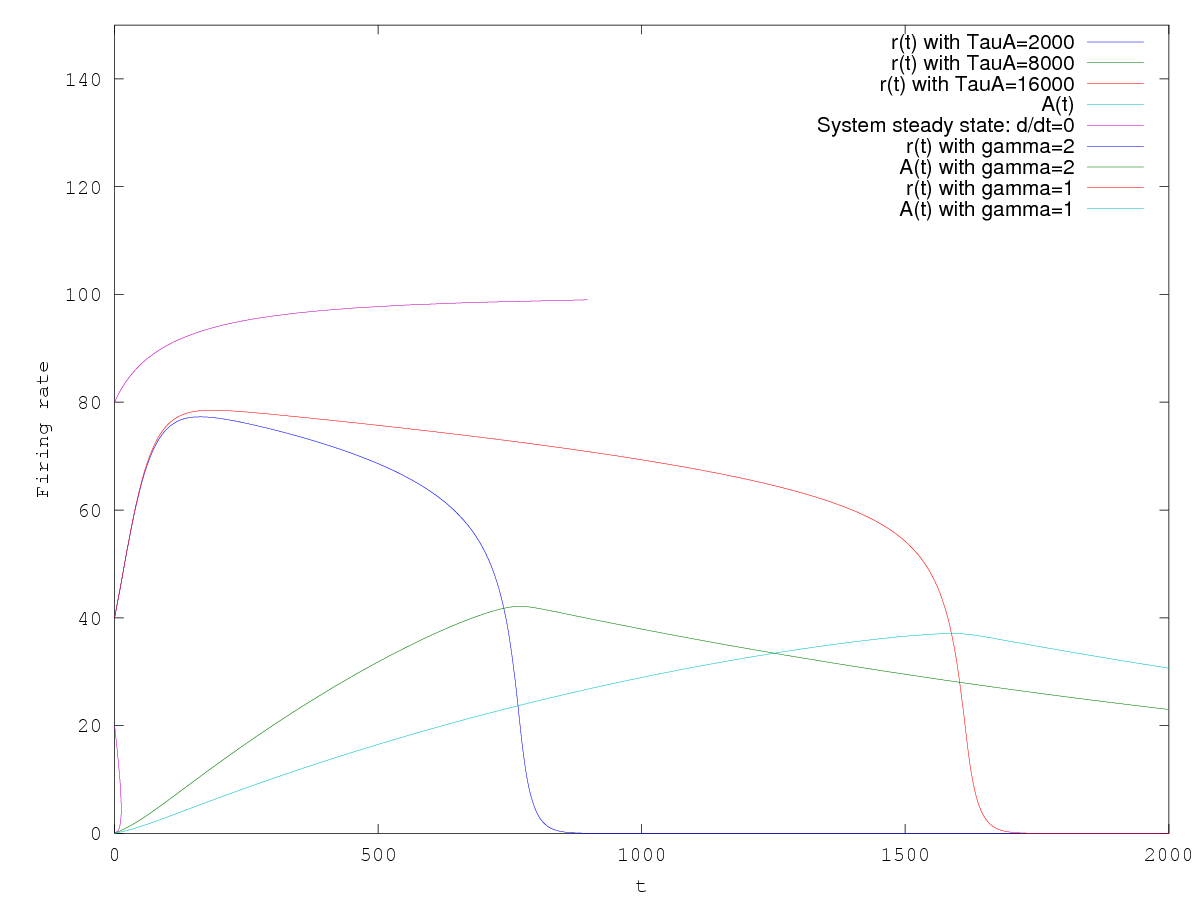
\includegraphics[width=6in]{1.png}\\
\section*{2}
For the second set of trials, I left $\gamma$ at $2$.  As I increased $\tau_A$, the system slowed down.  A(t) changed more slowly, so it took longer for A(t) to increase to drive R(t) down, and it took longer for A(t) do decrease again after R(t) plummeted.  The shape of the curves was qualitatively similar, however.\\
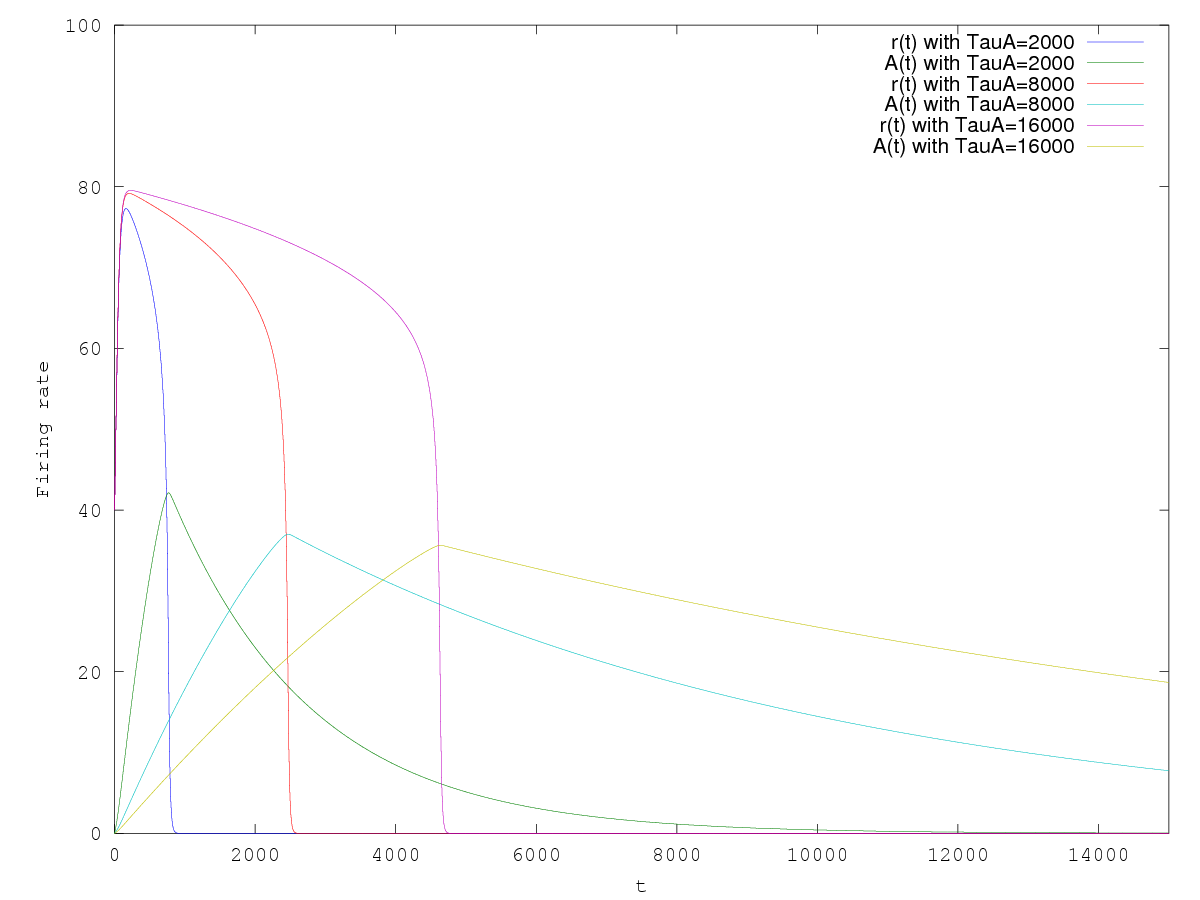
\includegraphics[width=6in]{2.png}\\

\newpage
\section*{3}
I approached finding the steady state curve analytically for individual values of r.  Given:
$\tau(dr/dt) = -r + S_{NR}(ar - A)$ (I = 0), we can set $dr/dt$ to 0 and calculate from there.
\begin{align*}
  r &= S_{NR}(ar-A)\\
  r &= \frac{M*(ar-A)^2}{\sigma^2 + (ar-A)^2}\\
  \delta &= (ar - A)^2\\
  r &= \frac{M*\delta}{\sigma^2 + \delta}\\
  r\sigma^2 + r\delta &= M*\delta\\
  \frac{r\sigma^2}{\delta} &= M-r\\
  \frac{1}{\delta} &= \frac{M-r}{r\sigma^2}\\
  \delta &= \frac{r\sigma^2}{M-r}\\
  A^2 - 2arA + a^2r^2 - \frac{r\sigma^2}{M-r} &= 0\\
\end{align*}
Since everything other than A is constant for a given r, this is a quadratic in A, easily solved.
In the graphs below, we can see R jump to the upper part of the steady state,
stay there for a little while as A(t) grows (STM), 
then fall to the bottom as A(t) dominates the input.
When $\tau_A$ is lowest, we can see A(t) immediately forcing
down r(t), so it doesn't spend much time at the top of the graph,
but as we raise $\tau_A$, r(t) remains for much of A(t)'s rise.\\
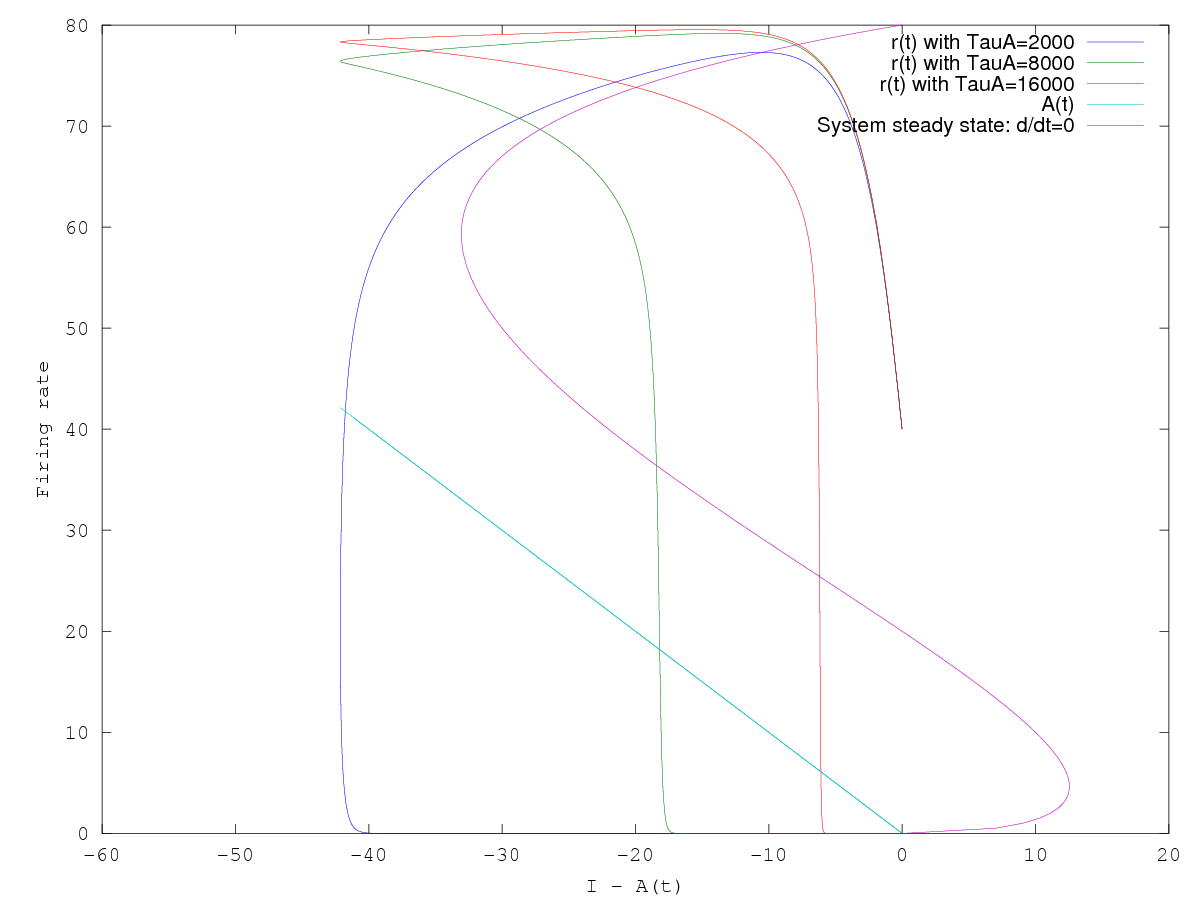
\includegraphics[width=6in]{3.png}\\

\section*{4}
For varying the values of I, I set $\tau_A$ back to 2000.
In these time courses, instead of the firing rate falling
to nothing, the constant input current causes the neuron
to reach a steady state solid firing rate.
The steady state is about 62 for I=30, 72 for I=50,
and 78 for I=70.
For any given I, we could find what steady state it would 
go to by first checking the sign of $dr/dt$,
to know whether it would go to a zero or positive steady state,
then if $dr/dt>0$, we can solve for r in $r=S_{NA}(ar-A(r))$.\\
In the six graphs below, we can see that the system oscillates
for each of these values of I, fastest for I=50, slightly slower
for I=70 since A is greater, and slowest for I=30.
In the phase planes, we can see that for each input value, 
the firing rate first jumps upwards, then goes into a cycle of
slowly decreasing as the input decreases, falling fast as A(t) rises,
then jumping again as A(t) falls.\\
\newpage
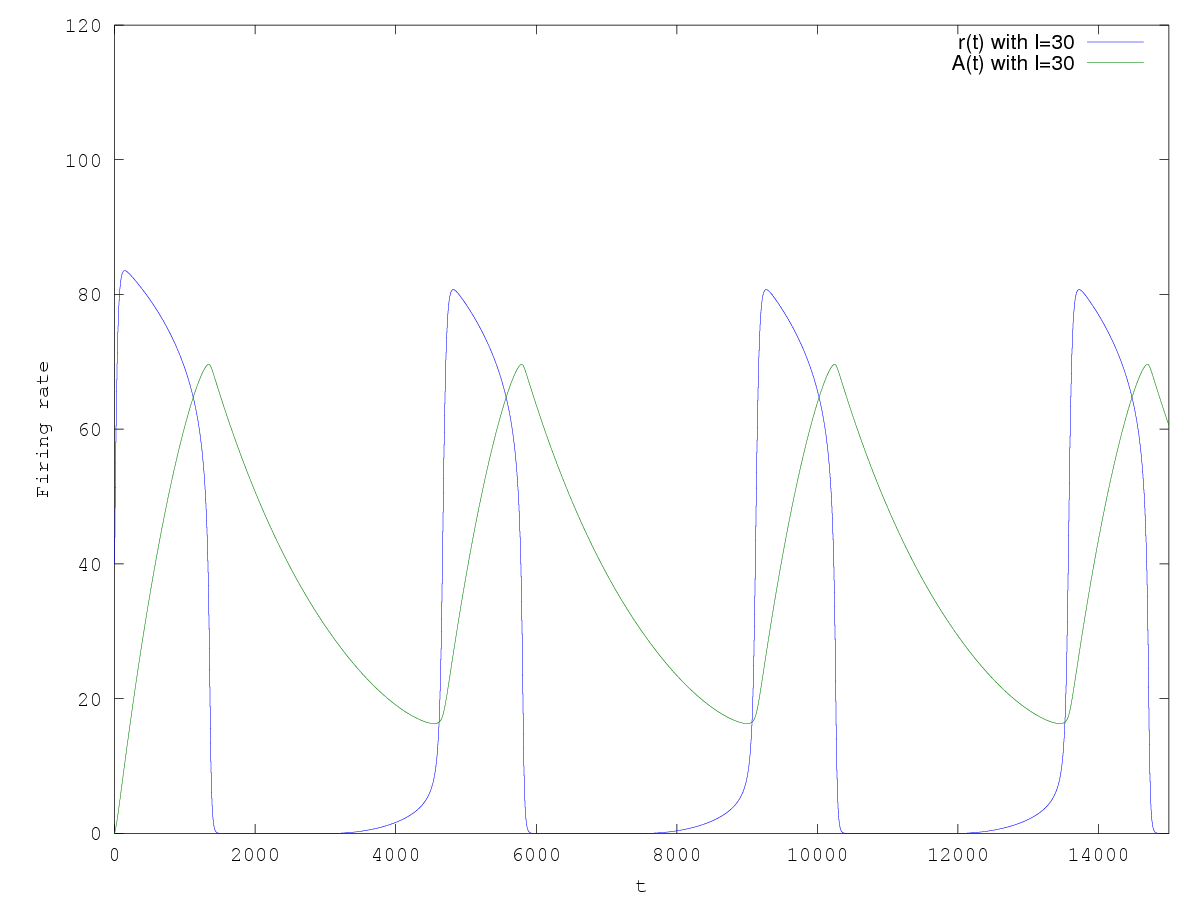
\includegraphics[width=5in]{4ta.png}\\
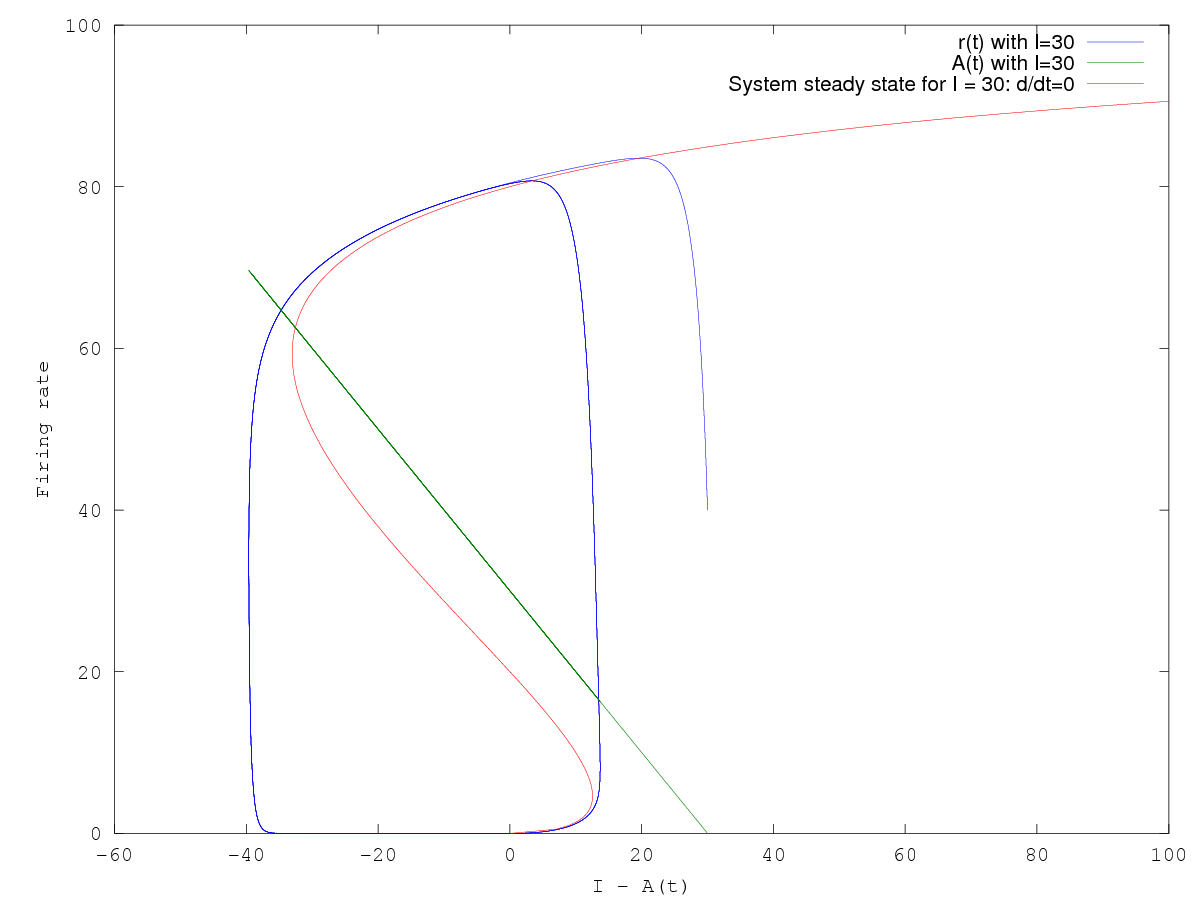
\includegraphics[width=5in]{4pa.png}\\
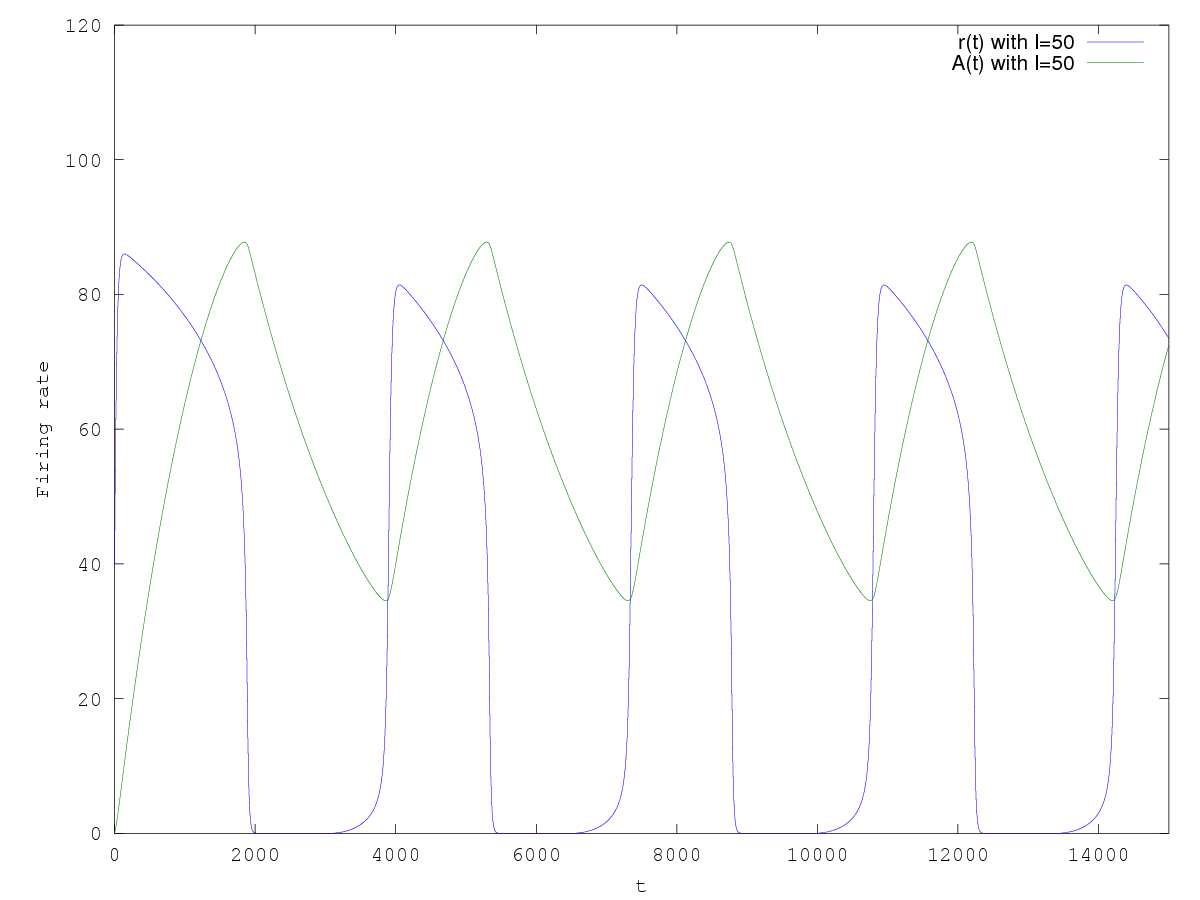
\includegraphics[width=5in]{4tb.png}\\
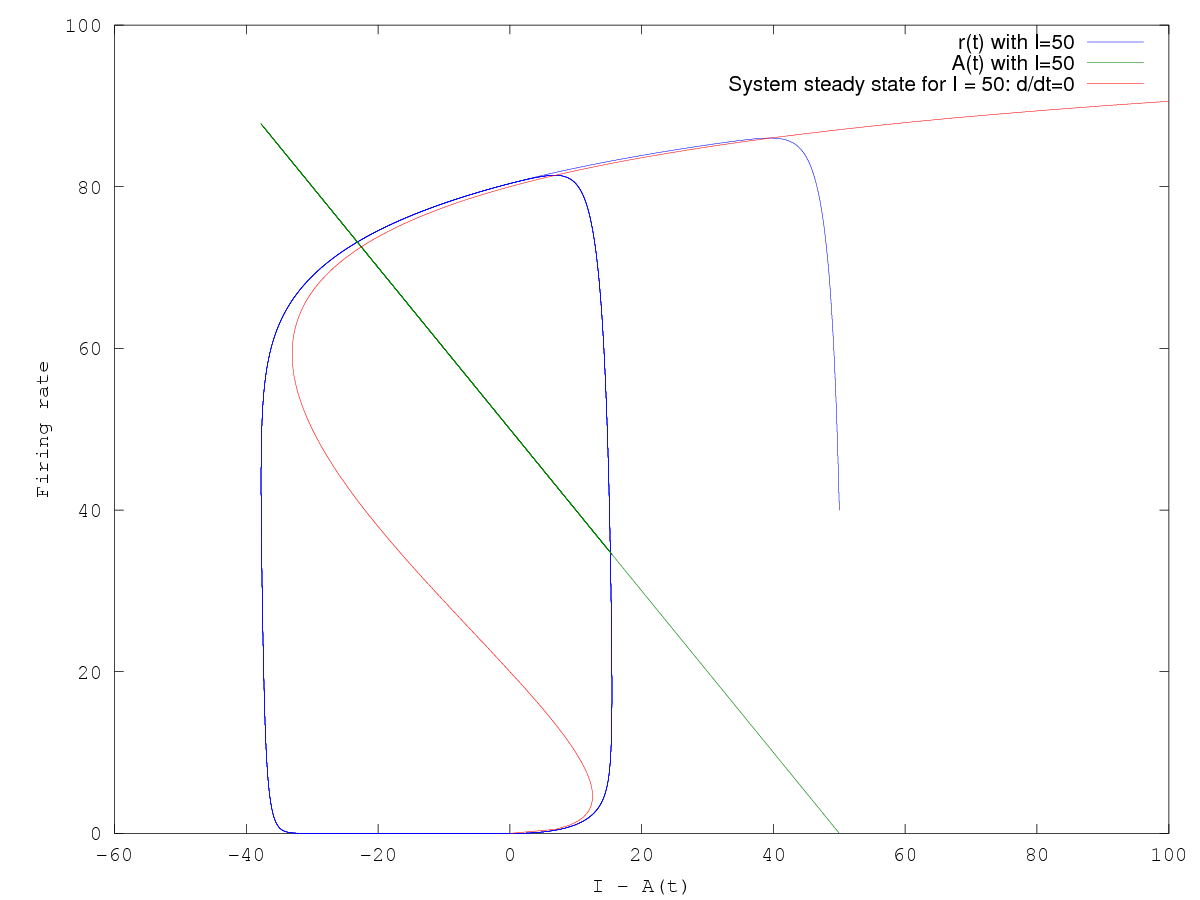
\includegraphics[width=5in]{4pb.png}\\
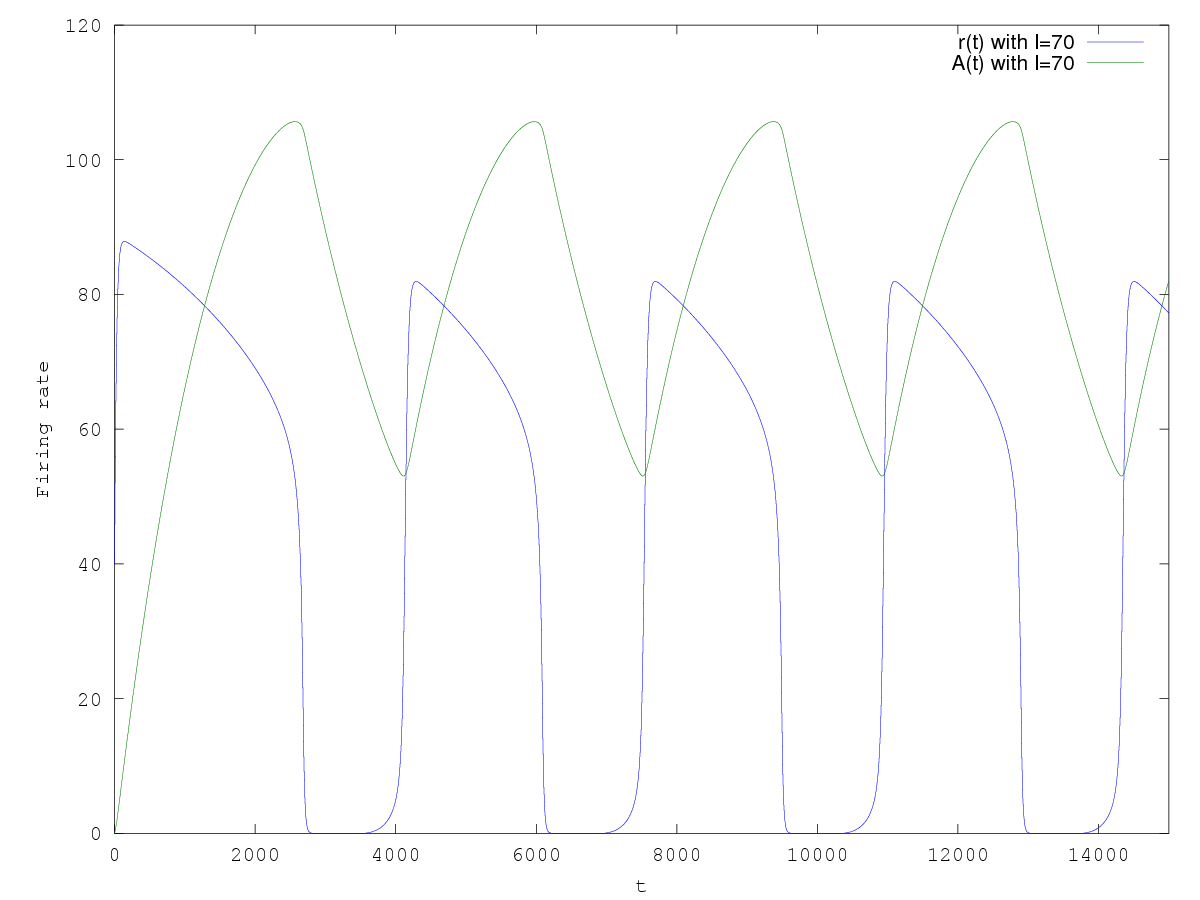
\includegraphics[width=5in]{4tc.png}\\
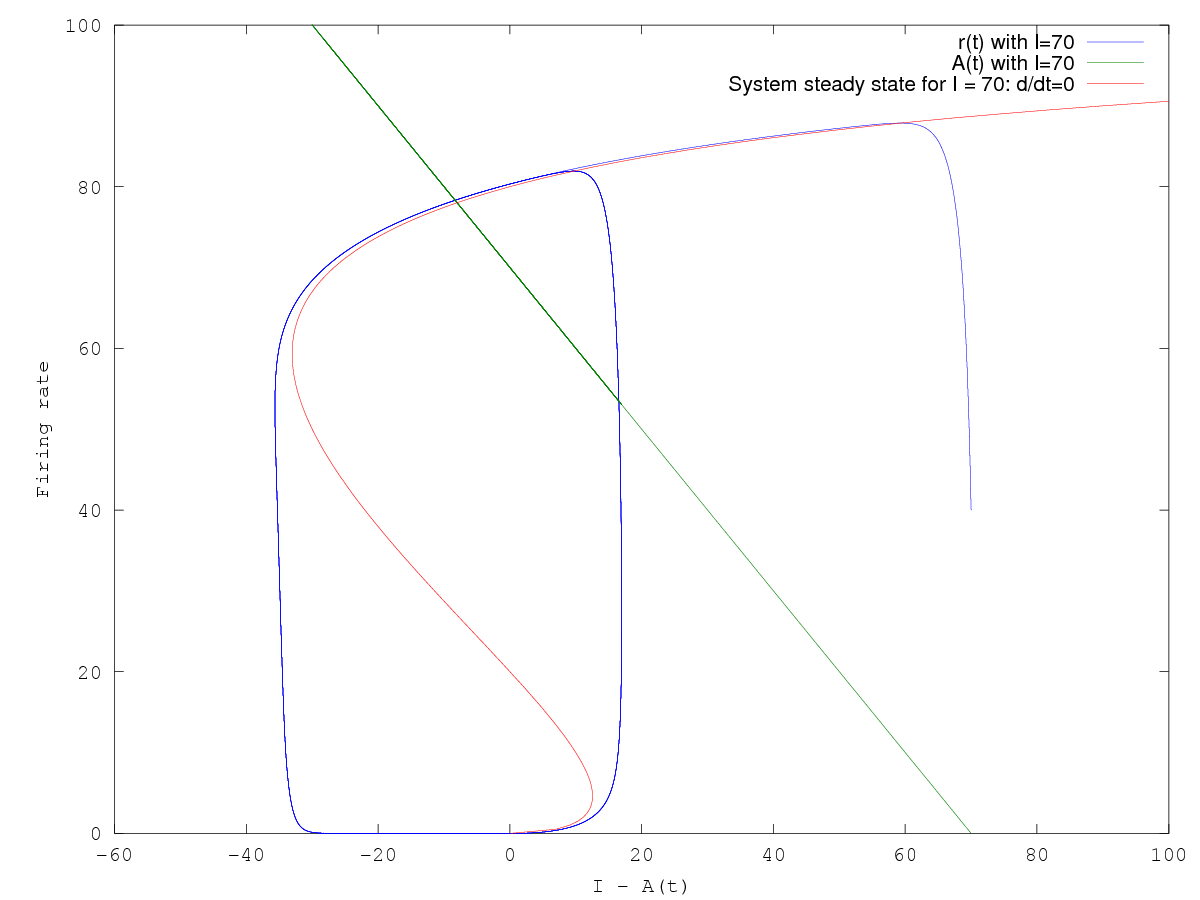
\includegraphics[width=5in]{4pc.png}\\
In order to find the threshold where the oscillating regime ends
and a forced constant firing rate begins,
I hypothesized that r(t) would stabilize
at the left side of the upper part of the steady state curve.
Then, to stop oscillation, I tried to choose an $I$ such that
$dA/dt = 0$ when $r(t) \approx 60$. 
Taking $dA/dt = 0$ gives $A = \gamma r=2r$, so A should stabilize at about $A=120$.
Then, since we know $dr/dt=0$, we can look at that equation.
\begin{align*}
r &= S_{NA}(ar+I-A)\\
60 &= S_{NA}(180+I-120)\\
60 &= S_{NA}(60+I)\\
60 &= S_{NA}(60+I)\\
60 &= \frac{M*(60+I)^2}{\sigma^2 + (60 + I)^2}\\
60 &= \frac{100*(60+I)^2}{120^2 + (60 + I)^2}\\
60 &= \frac{100*(60+I)^2}{120^2 + (60 + I)^2}\\
0 &= 40I^2 + 4800I -720000 \\
I &\approx 87\\
\end{align*}
I looked in the region around $I=87$, and found that
the regime change actually happens between $I=85$ and $I=86$.\\
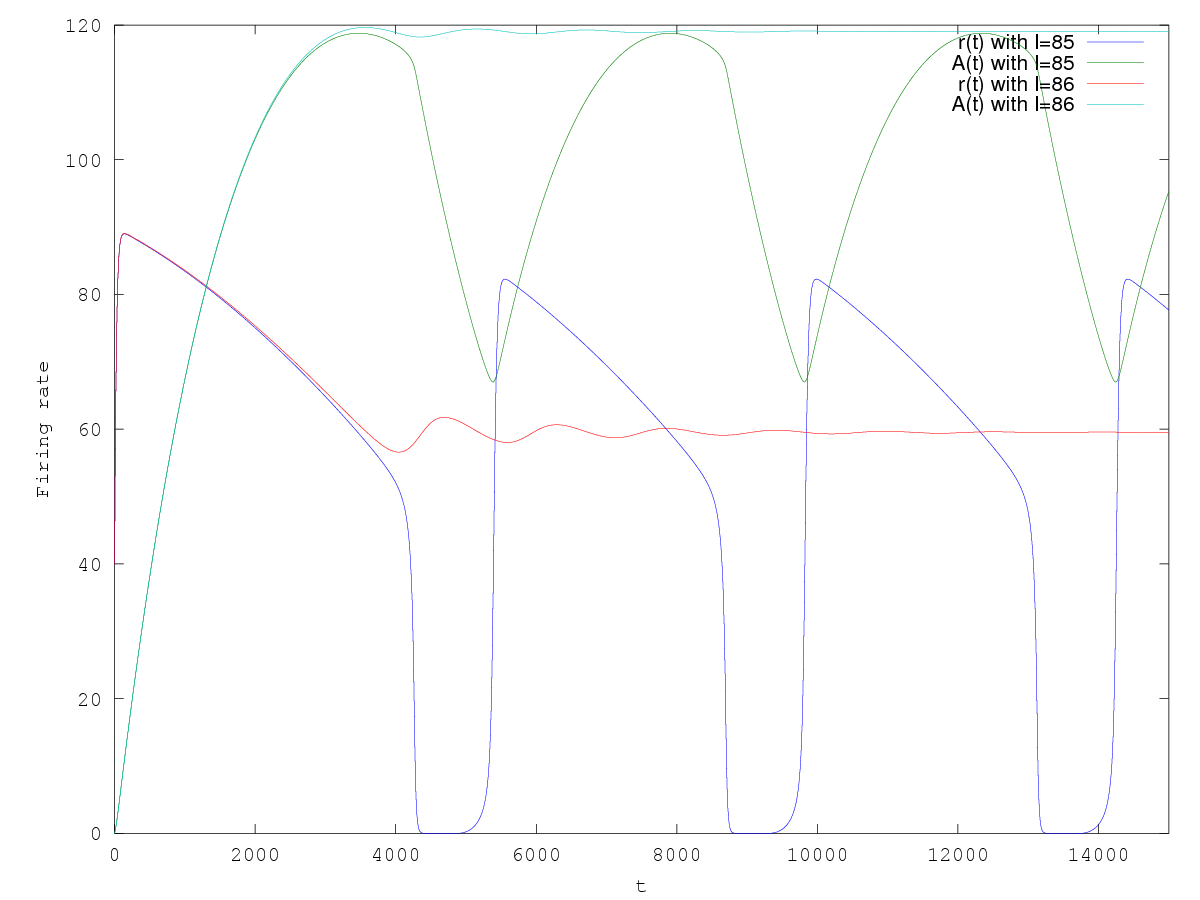
\includegraphics[width=6in]{5.png}\\
\end{document}
